% Options for packages loaded elsewhere
\PassOptionsToPackage{unicode}{hyperref}
\PassOptionsToPackage{hyphens}{url}
\PassOptionsToPackage{dvipsnames,svgnames,x11names}{xcolor}
%
\documentclass[
  letterpaper,
  DIV=11,
  numbers=noendperiod]{scrartcl}

\usepackage{amsmath,amssymb}
\usepackage{iftex}
\ifPDFTeX
  \usepackage[T1]{fontenc}
  \usepackage[utf8]{inputenc}
  \usepackage{textcomp} % provide euro and other symbols
\else % if luatex or xetex
  \usepackage{unicode-math}
  \defaultfontfeatures{Scale=MatchLowercase}
  \defaultfontfeatures[\rmfamily]{Ligatures=TeX,Scale=1}
\fi
\usepackage{lmodern}
\ifPDFTeX\else  
    % xetex/luatex font selection
  \setmainfont[]{Times new roman}
  \setmonofont[]{Times new roman}
\fi
% Use upquote if available, for straight quotes in verbatim environments
\IfFileExists{upquote.sty}{\usepackage{upquote}}{}
\IfFileExists{microtype.sty}{% use microtype if available
  \usepackage[]{microtype}
  \UseMicrotypeSet[protrusion]{basicmath} % disable protrusion for tt fonts
}{}
\makeatletter
\@ifundefined{KOMAClassName}{% if non-KOMA class
  \IfFileExists{parskip.sty}{%
    \usepackage{parskip}
  }{% else
    \setlength{\parindent}{0pt}
    \setlength{\parskip}{6pt plus 2pt minus 1pt}}
}{% if KOMA class
  \KOMAoptions{parskip=half}}
\makeatother
\usepackage{xcolor}
\setlength{\emergencystretch}{3em} % prevent overfull lines
\setcounter{secnumdepth}{5}
% Make \paragraph and \subparagraph free-standing
\ifx\paragraph\undefined\else
  \let\oldparagraph\paragraph
  \renewcommand{\paragraph}[1]{\oldparagraph{#1}\mbox{}}
\fi
\ifx\subparagraph\undefined\else
  \let\oldsubparagraph\subparagraph
  \renewcommand{\subparagraph}[1]{\oldsubparagraph{#1}\mbox{}}
\fi


\providecommand{\tightlist}{%
  \setlength{\itemsep}{0pt}\setlength{\parskip}{0pt}}\usepackage{longtable,booktabs,array}
\usepackage{calc} % for calculating minipage widths
% Correct order of tables after \paragraph or \subparagraph
\usepackage{etoolbox}
\makeatletter
\patchcmd\longtable{\par}{\if@noskipsec\mbox{}\fi\par}{}{}
\makeatother
% Allow footnotes in longtable head/foot
\IfFileExists{footnotehyper.sty}{\usepackage{footnotehyper}}{\usepackage{footnote}}
\makesavenoteenv{longtable}
\usepackage{graphicx}
\makeatletter
\def\maxwidth{\ifdim\Gin@nat@width>\linewidth\linewidth\else\Gin@nat@width\fi}
\def\maxheight{\ifdim\Gin@nat@height>\textheight\textheight\else\Gin@nat@height\fi}
\makeatother
% Scale images if necessary, so that they will not overflow the page
% margins by default, and it is still possible to overwrite the defaults
% using explicit options in \includegraphics[width, height, ...]{}
\setkeys{Gin}{width=\maxwidth,height=\maxheight,keepaspectratio}
% Set default figure placement to htbp
\makeatletter
\def\fps@figure{htbp}
\makeatother

<style>

h3 {
  text-align: left;
}

.center h2 {
  text-align: center;
}

.center h3 {
  text-align: center;
  font-size: 1.25rem;
}

.left h2 {
  text-align: left;
}

.left h3 {
  text-align: left;
}
</style>
\KOMAoption{captions}{tableheading}
\makeatletter
\@ifpackageloaded{caption}{}{\usepackage{caption}}
\AtBeginDocument{%
\ifdefined\contentsname
  \renewcommand*\contentsname{Table of contents}
\else
  \newcommand\contentsname{Table of contents}
\fi
\ifdefined\listfigurename
  \renewcommand*\listfigurename{List of Figures}
\else
  \newcommand\listfigurename{List of Figures}
\fi
\ifdefined\listtablename
  \renewcommand*\listtablename{List of Tables}
\else
  \newcommand\listtablename{List of Tables}
\fi
\ifdefined\figurename
  \renewcommand*\figurename{Figure}
\else
  \newcommand\figurename{Figure}
\fi
\ifdefined\tablename
  \renewcommand*\tablename{Table}
\else
  \newcommand\tablename{Table}
\fi
}
\@ifpackageloaded{float}{}{\usepackage{float}}
\floatstyle{ruled}
\@ifundefined{c@chapter}{\newfloat{codelisting}{h}{lop}}{\newfloat{codelisting}{h}{lop}[chapter]}
\floatname{codelisting}{Listing}
\newcommand*\listoflistings{\listof{codelisting}{List of Listings}}
\makeatother
\makeatletter
\makeatother
\makeatletter
\@ifpackageloaded{caption}{}{\usepackage{caption}}
\@ifpackageloaded{subcaption}{}{\usepackage{subcaption}}
\makeatother
\ifLuaTeX
  \usepackage{selnolig}  % disable illegal ligatures
\fi
\usepackage{bookmark}

\IfFileExists{xurl.sty}{\usepackage{xurl}}{} % add URL line breaks if available
\urlstyle{same} % disable monospaced font for URLs
\hypersetup{
  colorlinks=true,
  linkcolor={blue},
  filecolor={Maroon},
  citecolor={Blue},
  urlcolor={Blue},
  pdfcreator={LaTeX via pandoc}}

\author{}
\date{}

\begin{document}

\renewcommand*\contentsname{Table of contents}
{
\hypersetup{linkcolor=}
\setcounter{tocdepth}{3}
\tableofcontents
}
::: \{layout-ncol=2\}

\subsection{Evaluación 2}\label{evaluaciuxf3n-2}

\subsubsection{Juan Carlos Gaviria Chaverra, Andrés Orlando López
Henao}\label{juan-carlos-gaviria-chaverra-andruxe9s-orlando-luxf3pez-henao}

\textbf{1. Título del experimento}

Influencia de la longitud de la mecha en la duración de la combustión de
las velas.

\textbf{2. Objetivos}

Evaluar cómo diferentes longitudes de mecha afectan la duración de la
combustión de las velas.

\textbf{3. Marco teórico}

Transfondo relevante o marco teórico: (a) relaciones teóricas, (b)
conocimiento y experiencia de expertos, (c) experimentos previos. ¿Dónde
se ubica este experimento en el estudio de algún proceso en el sistema?

\textbf{4. Variable respuesta}

Variable respuesta: Tiempo de combustión de la vela.

Valores usuales de operación: Entre 0 y 60 minutos.

Precisión de medición: Minutos.

Instrumento de medida: Cronómetro.

\textbf{5. Variable de control}

Listado de: (a) cada variable de control o explicativa o factor, (b) los
niveles y valores usuales de operación en los cuales el proceso de
realiza, su distribución y el rango de operación usual, (c) precisión o
rango en el cual se irá a configurar (en el experimento, no
necesariamente en las operaciones de la planta) y la precisión a la cual
será tomada y su instrumentación, (d) la configuración propuesta de los
niveles en el experimento, (e) el efecto predicho (al menos de manera
cualitativa) sobre cada una de las variables respuesta.

\textbf{6. Factores controlables}

Listado de: (a) cada variable o factor que se mantendrá constante en el
experimento, (b) el nivel deseado o permitido y el rango admisible de
variación,(c) la precisión o el rango en el cual se mediará, intrumento
de medida, (d) cómo se controlará y (e) el impacto esperado, si existe,
en cada variable respuesta.

\textbf{7. Factores no controlables}

Listado de: (a) cada factor de molestia, (b) precisión en la medida (si
es posible), (c) estrategia (p.ej. bloqueo, aleatorización, selección),
y (d) efectos anticipados.

\textbf{8. Interacciones}

Listado y etiquetado de las interacciones conocidas o sospechadas.

\textbf{9. Restricciones}

Listado de restricciones del experimento. Descripción detallada de la
ejecución de cada etapa del experimento. Métodos de medida, materiales,
duración, número de repeticiones y réplicas, unidades experimentales,
regiones no permitidas de experimentación, límites de aleatorización,
orden de la corridas o experimentos, costos del cambio de nivel o
variable, etc.

\textbf{10. Diseño}

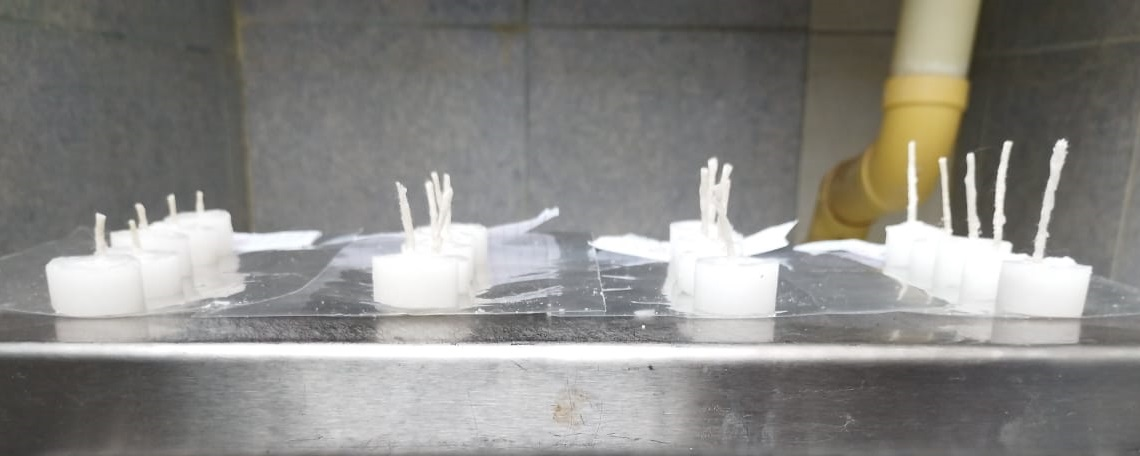
\includegraphics{imagenes/velas.jpeg}

\textbf{Diseño Experimental:} Se utilizará un diseño completamente
aleatorizado con cuatro niveles de mecha donde se mide el tiempo de
combustión de las velas.

\textbf{Factor:} Longitud de la mecha.

\textbf{Tratamientos:}

\begin{itemize}
\item
  \textbf{\emph{T1}}: Mecha 1 cm de longitud.
\item
  \textbf{\emph{T2}}: Mecha 1,5 cm longitud.
\item
  \textbf{\emph{T3}}: Mecha 2 cm longitud.
\item
  \textbf{\emph{T4}}: Mecha 2,5 cm longitud.
\end{itemize}

\textbf{Materiales:}

\begin{itemize}
\item
  Velas idénticas en tamaño y composición con mechas de diferentes
  longitudes.
\item
  Soportes para velas.
\item
  Cronómetro.
\item
  Encendedor.
\end{itemize}

\textbf{Procedimiento:}

\begin{itemize}
\item
  Cortar las mechas de manera uniforme en tres grupos con diferentes
  longitudes.
\item
  Fijar las mechas en las velas correspondientes según los grupos
  establecidos.
\item
  Encender cada vela al mismo tiempo y colocarlas en soportes idénticos.
\item
  Registrar el tiempo desde que se encienden hasta que se apagan por
  completo.
\item
  Repetir el experimento con varias velas para obtener datos
  adicionales.
\end{itemize}

\textbf{Análisis de Datos:} Comparar el tiempo promedio de combustión
entre los cuatro tipos de longitud de las mechas utilizando análisis
estadísticos, como el análisis de varianza (ANOVA) de un factor.

\textbf{Hipótesis:} Se espera que velas con mechas de mayor longitud
tengan una duración de combustión más larga.

\textbf{Resultados Esperados:} Se espera que las velas con mechas de
mayor longitud tengan una duración de combustión más larga en
comparación con las mechas de menor longitud, de acuerdo con la
hipótesis.

\textbf{11. Descripción}

Si es posible la descripción de la técnica de análisis y presentación.
Es decir gráficas, ANOVAS, regresión, estadísticos de prueba,
contrastes, etc.

\textbf{12. Responsable de coordinación}

Juan Carlos Gaviria Chaverra.

\textbf{13. Premuestreo}

No se realizará premuestreo por las siguientes razones:

Simplicidad del experimento: El diseño experimental es directo y no
implica procedimientos complicados. Consiste en encender velas con
diferentes longitudes de mecha y medir la duración de la combustión.
Dado que el procedimiento es simple y fácil de ejecutar, no se requiere
una fase preliminar de recolección de datos para ajustar o validar el
método experimental.

Condiciones experimentales bien definidas: Las condiciones del
experimento, como el ambiente de prueba y los materiales utilizados, son
conocidas y estables. Se llevará a cabo en un entorno controlado y las
velas utilizadas serán consistentes en calidad y composición. Por lo
tanto, se puede tener confianza en la replicabilidad de los resultados
sin la necesidad de un premuestreo para ajustar o validar estas
condiciones.

Recursos limitados: Los recursos disponibles, como tiempo, dinero y
personal, son limitados.

\textbf{14. Análisis}

\textbf{14.1 Datos}

\begin{verbatim}
# A tibble: 20 x 2
   Tratamientos Combustion
   <chr>             <dbl>
 1 T1_1cm             15.9
 2 T1_1cm             12.6
 3 T1_1cm             14.7
 4 T1_1cm             13.5
 5 T1_1cm             17.2
 6 T2_1.5cm           18.4
 7 T2_1.5cm           14.5
 8 T2_1.5cm           17.2
 9 T2_1.5cm           15.7
10 T2_1.5cm           20.1
11 T3_2cm             28.5
12 T3_2cm             22.5
13 T3_2cm             26.7
14 T3_2cm             24.3
15 T3_2cm             31.2
16 T4_2.5cm           31.4
17 T4_2.5cm           24.8
18 T4_2.5cm           29.4
19 T4_2.5cm           26.7
20 T4_2.5cm           34.4
\end{verbatim}

\textbf{14.2. Análisis gráfico}

\textbf{14.2.1. Histograma}

\begin{verbatim}
`stat_bin()` using `bins = 30`. Pick better value with `binwidth`.
\end{verbatim}

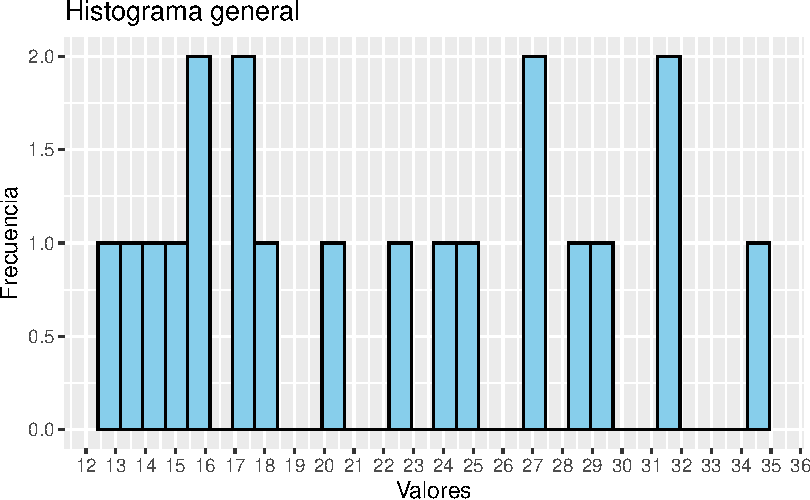
\includegraphics{Documento_files/figure-pdf/unnamed-chunk-2-1.pdf}

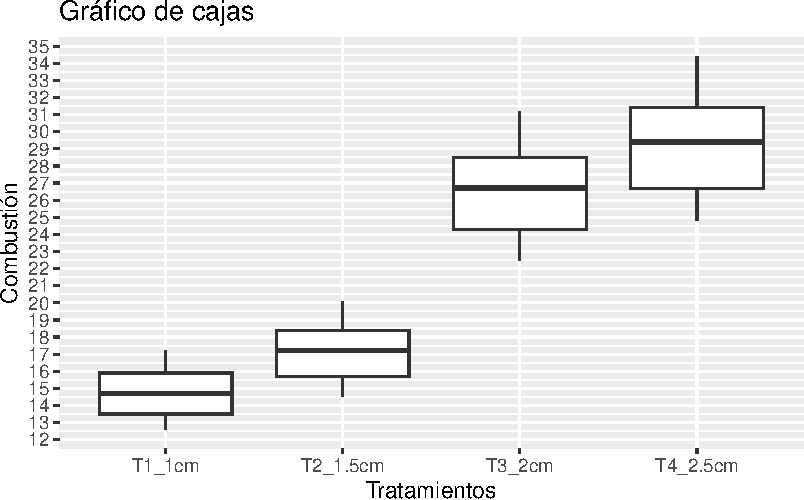
\includegraphics{Documento_files/figure-pdf/unnamed-chunk-3-1.pdf}

\textbf{14.3. Análisis estadístico}

\textbf{14.3.1. Análisis de normalidad}

\emph{H0:} El tiempo de combustión de las velas sigue una distribución
normal.

\emph{HA:} El tiempo de combustión de las velas no sigue una
distribución normal.

\textbf{14.3.1.1. Prueba de normalidad Shapiro-Wilk}

\begin{verbatim}

    Shapiro-Wilk normality test

data:  datos
W = 0.93093, p-value = 0.1609

La distribución de los datos es normal dado que el valor-p  0.1608868  es mayor que el nivel de confianza  0.05
\end{verbatim}

\textbf{14.3.1.2. Prueba de normalidad Jarque-Bera}

\begin{verbatim}

    Jarque-Bera Normality Test

data:  datos
JB = 1.5958, p-value = 0.4503
alternative hypothesis: greater

La distribución de los datos es normal dado que el valor-p  0.4502818  es mayor que el nivel de confianza  0.05
\end{verbatim}

\textbf{14.3.1.3. Prueba de normalidad Kolmogorov-Smirnov}

\begin{verbatim}

    Lilliefors (Kolmogorov-Smirnov) normality test

data:  datos
D = 0.15764, p-value = 0.2151

La distribución de los datos es normal dado que el valor-p  0.2151317  es mayor que el nivel de confianza  0.05
\end{verbatim}

\textbf{14.3.2. Análisis de normalidad tratamiento T1}

\emph{H0:} El tiempo de combustión de las velas del tratamiento T1 sigue
una distribución normal.

\emph{HA:} El tiempo de combustión de las velas del tratamiento T1 no
sigue una distribución normal.

\textbf{14.3.2.1. Prueba de normalidad Shapiro-Wilk}

\begin{verbatim}

    Shapiro-Wilk normality test

data:  datos
W = 0.97904, p-value = 0.9294

La distribución de los datos es normal dado que el valor-p  0.929427  es mayor que el nivel de confianza  0.05
\end{verbatim}

\textbf{14.3.2.2. Prueba de normalidad Jarque-Bera}

\begin{verbatim}

    Jarque-Bera Normality Test

data:  datos
JB = 0.38199, p-value = 0.8261
alternative hypothesis: greater

La distribución de los datos es normal dado que el valor-p  0.8261381  es mayor que el nivel de confianza  0.05
\end{verbatim}

\textbf{14.3.2.3. Prueba de normalidad Kolmogorov-Smirnov}

\begin{verbatim}

    Lilliefors (Kolmogorov-Smirnov) normality test

data:  datos
D = 0.15695, p-value = 0.9524

La distribución de los datos es normal dado que el valor-p  0.9523914  es mayor que el nivel de confianza  0.05
\end{verbatim}

\textbf{14.3.3. Análisis de normalidad tratamiento T2}

\emph{H0:} El tiempo de combustión de las velas del tratamiento T2 sigue
una distribución normal.

\emph{HA:} El tiempo de combustión de las velas del tratamiento T2 no
sigue una distribución normal.

\textbf{14.3.3.1. Prueba de normalidad Shapiro-Wilk}

\begin{verbatim}

    Shapiro-Wilk normality test

data:  datos
W = 0.98663, p-value = 0.9666

La distribución de los datos es normal dado que el valor-p  0.9666263  es mayor que el nivel de confianza  0.05
\end{verbatim}

\textbf{14.3.3.2. Prueba de normalidad Jarque-Bera}

\begin{verbatim}

    Jarque-Bera Normality Test

data:  datos
JB = 0.33754, p-value = 0.8447
alternative hypothesis: greater

La distribución de los datos es normal dado que el valor-p  0.8447024  es mayor que el nivel de confianza  0.05
\end{verbatim}

\textbf{14.3.3.3. Prueba de normalidad Kolmogorov-Smirnov}

\begin{verbatim}

    Lilliefors (Kolmogorov-Smirnov) normality test

data:  datos
D = 0.14928, p-value = 0.9716

La distribución de los datos es normal dado que el valor-p  0.9715818  es mayor que el nivel de confianza  0.05
\end{verbatim}

\textbf{14.3.4. Análisis de normalidad tratamiento T3}

\emph{H0:} El tiempo de combustión de las velas del tratamiento T3 sigue
una distribución normal.

\emph{HA:} El tiempo de combustión de las velas del tratamiento T3 no
sigue una distribución normal.

\textbf{14.3.4.1. Prueba de normalidad Shapiro-Wilk}

\begin{verbatim}

    Shapiro-Wilk normality test

data:  datos
W = 0.98538, p-value = 0.9612

La distribución de los datos es normal dado que el valor-p  0.9611567  es mayor que el nivel de confianza  0.05
\end{verbatim}

\textbf{14.3.4.2. Prueba de normalidad Jarque-Bera}

\begin{verbatim}

    Jarque-Bera Normality Test

data:  datos
JB = 0.3389, p-value = 0.8441
alternative hypothesis: greater

La distribución de los datos es normal dado que el valor-p  0.8441285  es mayor que el nivel de confianza  0.05
\end{verbatim}

\textbf{14.3.4.3. Prueba de normalidad Kolmogorov-Smirnov}

\begin{verbatim}

    Lilliefors (Kolmogorov-Smirnov) normality test

data:  datos
D = 0.15288, p-value = 0.9633

La distribución de los datos es normal dado que el valor-p  0.963337  es mayor que el nivel de confianza  0.05
\end{verbatim}

\textbf{14.3.5. Análisis de normalidad tratamiento T4}

\emph{H0:} El tiempo de combustión de las velas del tratamiento T4 sigue
una distribución normal.

\emph{HA:} El tiempo de combustión de las velas del tratamiento T4 no
sigue una distribución normal.

\textbf{14.3.5.1. Prueba de normalidad Shapiro-Wilk}

\begin{verbatim}

    Shapiro-Wilk normality test

data:  datos
W = 0.98332, p-value = 0.9516

La distribución de los datos es normal dado que el valor-p  0.9515727  es mayor que el nivel de confianza  0.05
\end{verbatim}

\textbf{14.3.5.2. Prueba de normalidad Jarque-Bera}

\begin{verbatim}

    Jarque-Bera Normality Test

data:  datos
JB = 0.34669, p-value = 0.8408
alternative hypothesis: greater

La distribución de los datos es normal dado que el valor-p  0.8408454  es mayor que el nivel de confianza  0.05
\end{verbatim}

\textbf{14.3.5.3. Prueba de normalidad Kolmogorov-Smirnov}

\begin{verbatim}

    Lilliefors (Kolmogorov-Smirnov) normality test

data:  datos
D = 0.15701, p-value = 0.9522

La distribución de los datos es normal dado que el valor-p  0.9522275  es mayor que el nivel de confianza  0.05
\end{verbatim}

\textbf{14.3.6. Comparación de medias entre dos poblaciones}

\textbf{14.3.7. Comparación de varianzas entre dos poblaciones}

\textbf{14.3.7.1. Comparación de varianzas T1 y T2}

\begin{verbatim}

    F test to compare two variances

data:  datos1 and datos2
F = 0.69672, num df = 4, denom df = 4, p-value = 0.7347
alternative hypothesis: true ratio of variances is not equal to 1
95 percent confidence interval:
 0.07254073 6.69166442
sample estimates:
ratio of variances 
         0.6967196 

[1] "Valor crítico1: 0.00108477764761528"
[1] "Valor crítico1: 10.0069821966136"
\end{verbatim}

\textbf{14.3.7.2. Comparación de varianzas T1 y T3}

\begin{verbatim}

    F test to compare two variances

data:  datos1 and datos2
F = 0.28819, num df = 4, denom df = 4, p-value = 0.2555
alternative hypothesis: true ratio of variances is not equal to 1
95 percent confidence interval:
 0.03000554 2.76792093
sample estimates:
ratio of variances 
         0.2881891 

[1] "Valor crítico1: 0.00108477764761528"
[1] "Valor crítico1: 10.0069821966136"
\end{verbatim}

\textbf{14.3.7.3. Comparación de varianzas T1 y T4}

\begin{verbatim}

    F test to compare two variances

data:  datos1 and datos2
F = 0.2352, num df = 4, denom df = 4, p-value = 0.1899
alternative hypothesis: true ratio of variances is not equal to 1
95 percent confidence interval:
 0.02448843 2.25898436
sample estimates:
ratio of variances 
         0.2351999 

[1] "Valor crítico1: 0.00108477764761528"
[1] "Valor crítico1: 10.0069821966136"
\end{verbatim}

\textbf{14.3.7.4. Comparación de varianzas T2 y T3}

\begin{verbatim}

    F test to compare two variances

data:  datos1 and datos2
F = 0.41364, num df = 4, denom df = 4, p-value = 0.4135
alternative hypothesis: true ratio of variances is not equal to 1
95 percent confidence interval:
 0.04306688 3.97279027
sample estimates:
ratio of variances 
         0.4136371 

[1] "Valor crítico1: 0.00108477764761528"
[1] "Valor crítico1: 10.0069821966136"
\end{verbatim}

\textbf{14.3.7.5. Comparación de varianzas T2 y T4}

\begin{verbatim}

    F test to compare two variances

data:  datos1 and datos2
F = 0.33758, num df = 4, denom df = 4, p-value = 0.3179
alternative hypothesis: true ratio of variances is not equal to 1
95 percent confidence interval:
 0.03514819 3.24231483
sample estimates:
ratio of variances 
         0.3375818 

[1] "Valor crítico1: 0.00108477764761528"
[1] "Valor crítico1: 10.0069821966136"
\end{verbatim}

\textbf{14.3.7.6. Comparación de varianzas T3 y T4}

\begin{verbatim}

    F test to compare two variances

data:  datos1 and datos2
F = 0.81613, num df = 4, denom df = 4, p-value = 0.8487
alternative hypothesis: true ratio of variances is not equal to 1
95 percent confidence interval:
 0.08497349 7.83854863
sample estimates:
ratio of variances 
         0.8161304 

[1] "Valor crítico1: 0.00108477764761528"
[1] "Valor crítico1: 10.0069821966136"
\end{verbatim}

\textbf{14.3.8. Modelo de medias}

\textbf{14.3.9. Modelo de efectos}

\textbf{14.3.10. Modelo de regresión}

\textbf{14.3.11. Tabla ANOVA}

\begin{verbatim}
                   Df Sum Sq Mean Sq F value  Pr(>F)    
datos$Tratamientos  3  753.8  251.28    29.3 9.8e-07 ***
Residuals          16  137.2    8.58                    
---
Signif. codes:  0 '***' 0.001 '**' 0.01 '*' 0.05 '.' 0.1 ' ' 1
\end{verbatim}

\begin{verbatim}
  Tukey multiple comparisons of means
    95% family-wise confidence level

Fit: aov(formula = datos$Combustion ~ datos$Tratamientos, data = datos)

$`datos$Tratamientos`
                   diff       lwr       upr     p adj
T2_1.5cm-T1_1cm    2.40 -2.898683  7.698683 0.5784494
T3_2cm-T1_1cm     11.86  6.561317 17.158683 0.0000470
T4_2.5cm-T1_1cm   14.56  9.261317 19.858683 0.0000038
T3_2cm-T2_1.5cm    9.46  4.161317 14.758683 0.0005507
T4_2.5cm-T2_1.5cm 12.16  6.861317 17.458683 0.0000351
T4_2.5cm-T3_2cm    2.70 -2.598683  7.998683 0.4839575
\end{verbatim}

4



\end{document}
